%% V1.0
%% by Gabriel Garcia, gabrcg@gmail.com
%% This is a template for Udacity projects using IEEEtran.cls

%% Be Udacious!

\documentclass[10pt,journal,compsoc]{IEEEtran}

\usepackage[pdftex]{graphicx}    
\usepackage{cite}
\usepackage[inline]{enumitem}
\usepackage{subfigure}
\usepackage{hyperref}
\usepackage{algorithmic}
\usepackage{algorithm}
\hyphenation{op-tical net-works semi-conduc-tor}


\begin{document}

\title{Where Am I?}

\author{Saminda Abeyruwan}

\markboth{Where Am I project, Robotic Nanodegree, Udacity}%
{}
\IEEEtitleabstractindextext{%

\begin{abstract}

Mobile robot localization estimates the robot pose relative to a given map of the environment. This project empirically evaluates the Adaptive Monte Carlo Localization algorithm using Gazebo simulator and RViz visualizer. Using ROS framework, a baseline two- and custom four-wheeled mobile robot platforms with senors have been developed. The robots have used ROS amcl and navigation stack packages for global localization and path planning. By tuning the amcl and planner parameters, the robots have been localized on the map and successfully navigated to predefined target locations. 
\end{abstract}

% Note that keywords are not normally used for peerreview papers.
\begin{IEEEkeywords}
Robot, IEEEtran, Udacity, \LaTeX, deep learning.
\end{IEEEkeywords}}


\maketitle
\IEEEdisplaynontitleabstractindextext
\IEEEpeerreviewmaketitle
\section{Introduction}
\label{sec:introduction}

\IEEEPARstart{M}{bile} robot localization estimates the robot pose relative to a given  map of the environment \cite{Thrun:2005:PR:1121596}. Given the coordinates of the map, a robot pose, $x_t = (x~ y~\theta)^T$, sufficiently determines location and orientation of the robot. The robot pose cannot be directly sensed, and it must be inferred from the noisy sensor data over time. There are four dimensions with which the complexity of the localization problems can be analyzed. 

The first dimension is based on the knowledge available initially, and during the operation time.  There are three complexity classes; \begin{enumerate*} \item \textit{position tracking}, the initial pose of the robot is known, and the localization is achieved via accommodating the noisy robot motion. If the motion error is relatively small, the pose uncertainty is often approximated by a unimodal distribution.  This is also a local localization, as the pose is confined to a small region of the robot true pose, \item \textit{global localization}, the initial pose of the robot is unknown, and it is inferred from relative to a known map of the environment. The problem is  more difficult than position tracking, and generally cannot be bounded by a a unimodal distribution, and \item \textit{kidnapped robot problem}, the robot gets teleported to some other location. The robot needs to reevaluate its pose, and recover from such situations to exhibits truly autonomous capabilities. \end{enumerate*} 

The second dimension addresses the nature of the environment: \begin{enumerate*} \item \textit{static environments}, the objects in the environment remain static, and the only variable is the robot pose, and \item \textit{dynamic environments}, contains objects whose location of configuration changes overtime.  \end{enumerate*}

The third dimension addresses the ability of the localization algorithms to control the motion of the robot. There are two modes: \begin{enumerate*} \item \textit{passive localization}, where the localization module only observes the sensor and motion readings, and the robot is controlled by another set of modules, and \item \textit{active localization}, controls the robot to minimize the localization error.  \end{enumerate*} 

\begin{figure}[thpb]
      \centering
      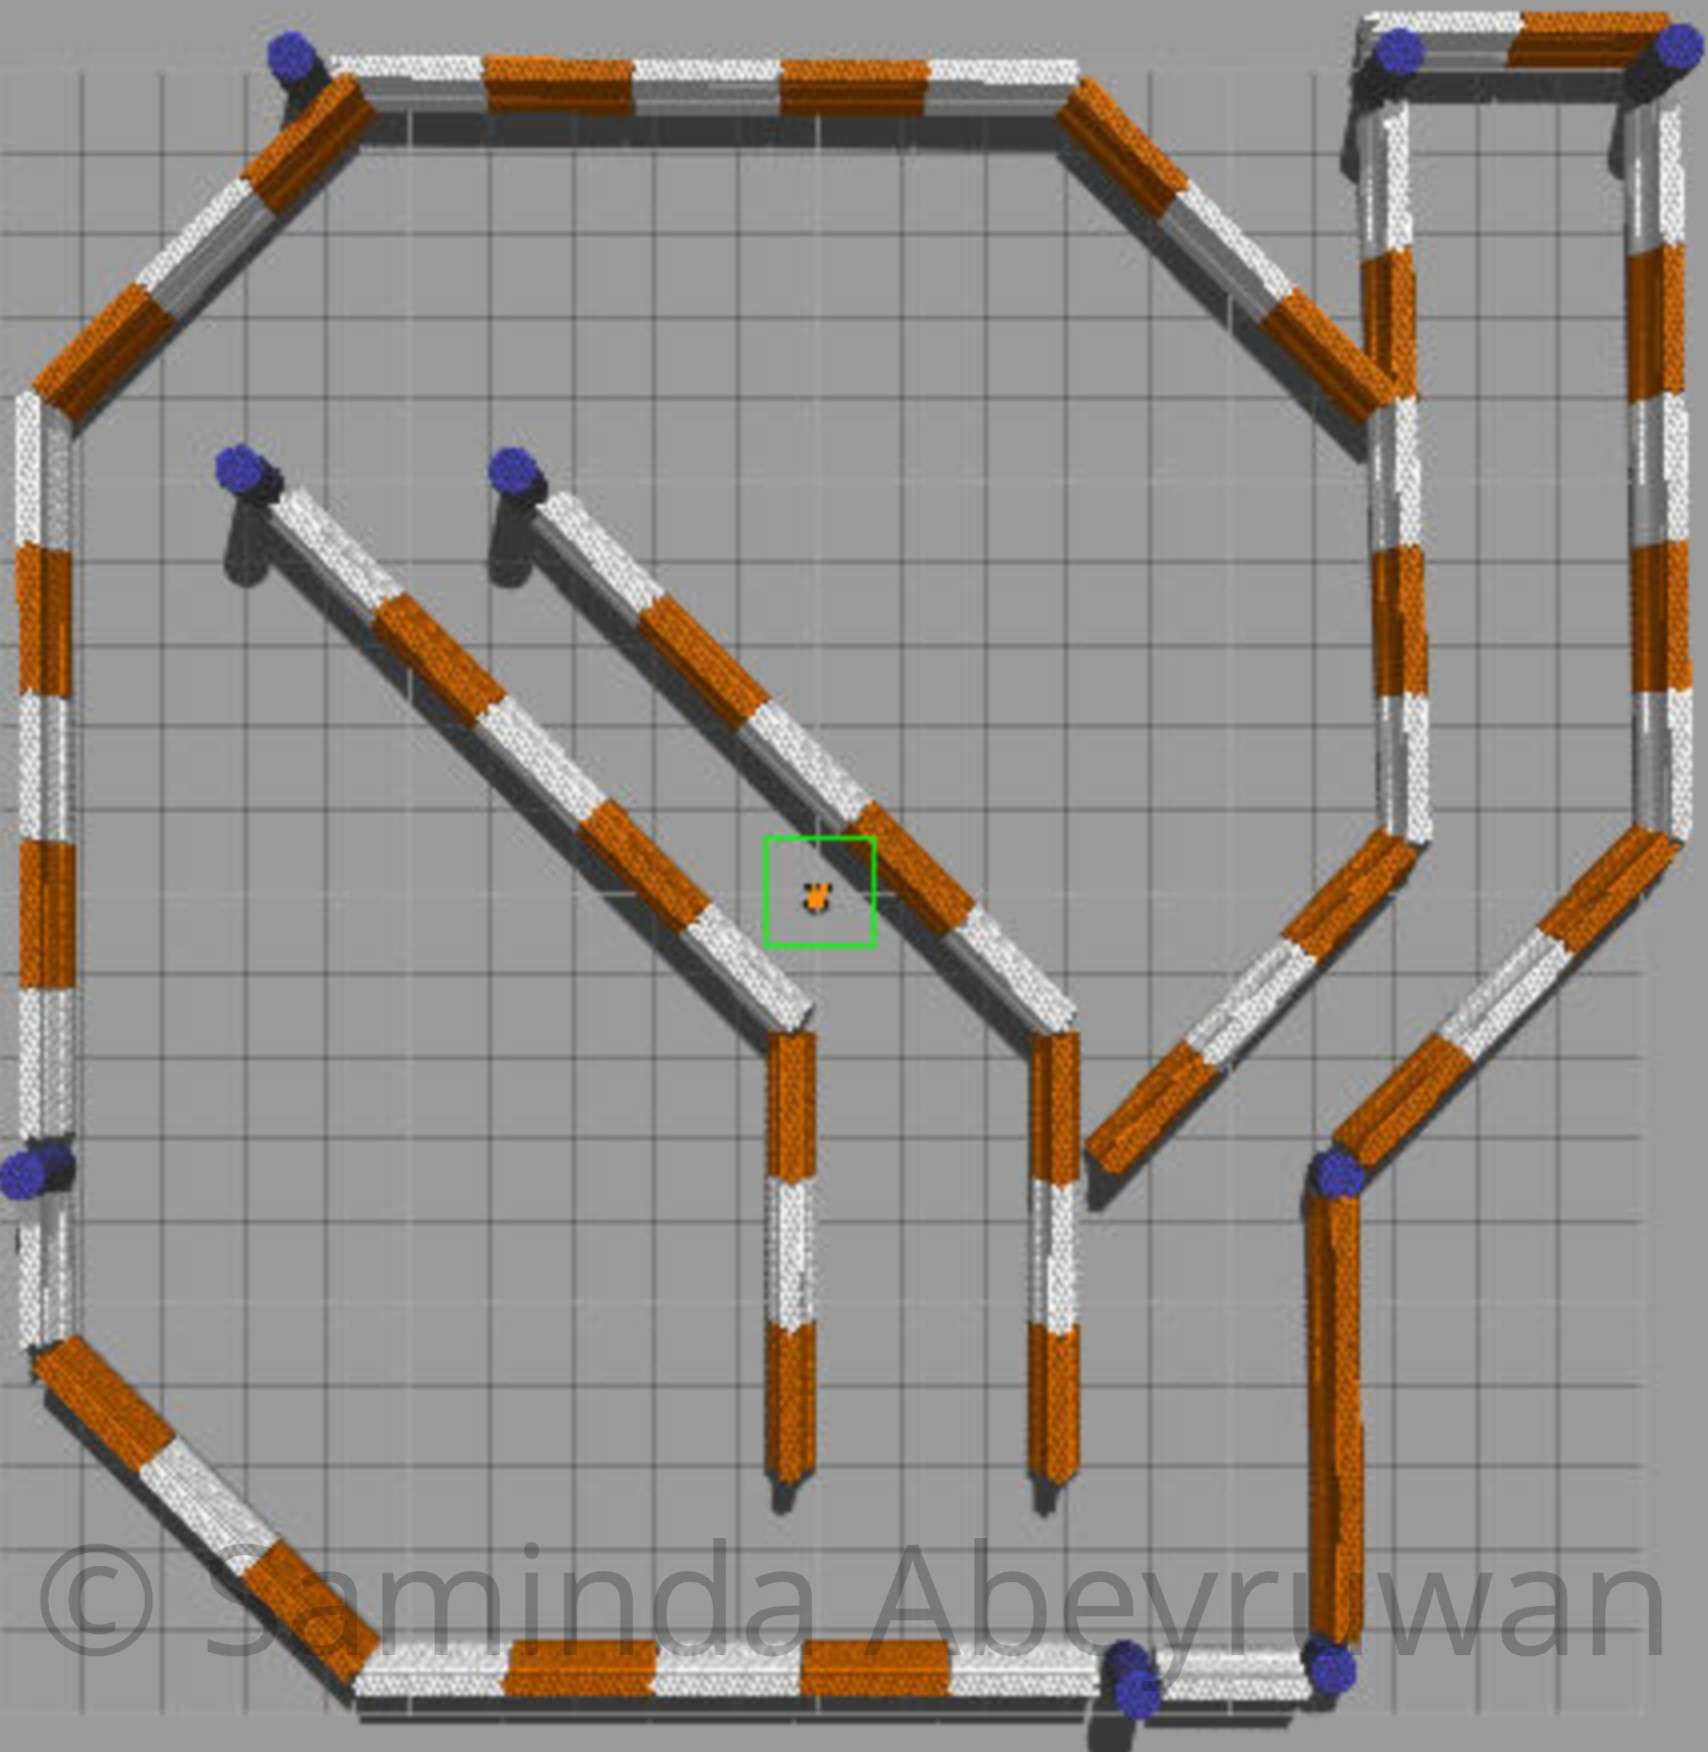
\includegraphics[width=\linewidth]{misc/map_w.png}
      \caption{Jackal race static map of the environment.}
      \label{fig:map}
\end{figure}

Finally, last dimension involved the number of robots involved: \begin{enumerate*} \item \textit{single-robot localization}, all sensor and motion information is collected from a single robot platform, and \item \textit{multi-robot localization}, information from other robots in a team of robots are used to solve the localization problem. \end{enumerate*}

This project is focused on solving the global localization problem on a static environment, using a passive module, in a single-robot mobile platform. This has been implemented in simulation via ROS \cite{288} packages to illustrate navigation tasks (Fig. \ref{fig:map}).  


%example for inserting image
%\begin{figure}[thpb]
%      \centering
%      \includegraphics[width=\linewidth]{RobotRevolution5}
%      \caption{Robot Revolution.}
%      \label{fig:robot1}
%\end{figure}

%\subsection{Subsection Heading Here}
%Subsection text here.
%
%\subsubsection{Subsubsection Heading Here}
%Subsubsection text here.
%
%
%\begin{table}[h]
%\caption{Table}
%\label{table_example}
%\begin{center}
%\begin{tabular}{|c||c|}
%\hline
%One & Two\\
%\hline
%Three & Four\\
%\hline
%\end{tabular}
%\end{center}
%\end{table}


\section{Background}

In global localization, the robot is placed within a known environment and localizes itself relative to an external reference frame. Due to the inherent uncertainty in sensor and motion measurements, the robot pose is represented by a \textit{belief}, a probability density function over the all possible locations and orientation.  Markov localization, an extension of the Bayes filter, provides a framework to obtain the robot pose as shown in the  Alg. \ref{alg:markov_localization}. 

\begin{algorithm}
\caption{Markov\_localization ($bel(x_{t-1}), u_t, z_t, m$)}\label{euclid}
\label{alg:markov_localization}
\begin{algorithmic}
\STATE  $\forall x_t$\textbf{:}
\STATE ~~~$\overline{bel}(x_t) = \int p(x_t | u_t, x_{t-1}, m)~bel(x_{t-1})~ dx_{t-1}$
\STATE ~~~$bel(x_t) = \eta~p(z_t | x_t, m)~\overline{bel}(x_t)$
\STATE \textbf{return} $bel(x_t)$
\end{algorithmic}
\end{algorithm}

The belief of the robot at time $t$ is represented by $bel(x_t)$. The measurement model and the motion model is given by $p(z_t | x_t, m)$, and $p(x_t | u_t, x_{t-1}, m)$ respectively. $u_t$ provides the control command to move the robot from time $t$-$1$ to t, while $z_t$ is the measurement, and $m$ is the static map of the environment. Kalman filter and Monte Carlo localization are two specific instances of the realization of the Alg. \ref{alg:markov_localization}, and further discussed herewith.   

\subsection{Kalman Filter Localization}
\label{sub:kfl}

The Kalman filter (KF) localization is a specific instance of Alg. \ref{alg:markov_localization}, the belief, measurement, and motion models are represented by the first (mean) and second (covariance) moments.  These assumptions limit the motion and measurement models to be linear, and the belief can only be represented by unimodal distribution such as a Gaussian. 

The practical systems are inherently non-linear, and the two common filters used in practice are the Extended Kalman filter (EKF), and the Unscented Kalman filter (UKF) localization. The EKF uses Taylor seriese expansion to linearize the non-linear model equations, while UKF uses sigma points for the transformation.  EKF and UKF localization represent with unimodal Gaussian and it is a good representation in uncertainty  for tracking problems, but generally not suitable for global localization. While  both algorithms addresses the limitation of the KF, the implementations use considerable computation resources (please refer to \cite{Thrun:2005:PR:1121596}, chapter 7, for comprehensive description of the filters).   

\subsection{Monte Carlo Location}
\label{sub:mcl}

Monte Carlo Localization (MCL) represents the belief $bel(x_t)$ of the robot pose by particles, which is a popular algorithm used in global and kidnapped robot localization.  MCL is computationally efficient than EKF and UKF, and it is not subjected to assumptions outlined in Sec. \ref{sub:kfl}. The basic steps of the MCL algorithm are:   \begin{enumerate*} \item the initial global uncertainty is achieved via a set of pose particles sampled uniform randomly over the entire pose space, \item the motion model moves the particles to the new locations, \item the measurement model assigns important factors to each particle based on the observations, \item the resampling setp samples particles relative to the importance weighs, and obtain the new belief, and set the new particles to uniform importance weights.  \end{enumerate*}

This project uses Adaptive Monte Carlo Localization  (AMCL) algorithm, which is a variant of MCL, that uses Kullback-Leibler divergence (KDL)-sampling to adapt the size of the particle set over time. 

\subsection{Practical Considerations}

Table \ref{tab:comp} summarizes and compares the localization algorithms discussed in Sec. \ref{sub:kfl} and \ref{sub:mcl}. While EKF and UKF are improvements over KF, they do come with limiting assumptions, and usage of considerable computational resources. On the other hand MCL and its variants can be used to represent multimodal distributions, and provide the ability to allocate proper computational resources.    

\begin{table}[h]
\caption{Comparison of EKF, UKF and MCL implementations}
\label{tab:comp}
\begin{center}
\begin{tabular}{|l||l|l|}
\hline
& EKF/UKF & MCL\\
\hline
Measurement & landmarks & row measurements\\
Measurement noise  & Gaussian & any\\
Posterior & Gaussian & particles\\
Efficiency (memory) & ++ &+\\
Efficiency (time) & ++ & +\\
Ease of implementation & + & ++\\
Resolution & ++ & +\\
Robustness & - & ++\\
Global localization & no & yes\\
\hline
\end{tabular}
\end{center}
\end{table}




%
%%example for Bullet point list
%
%\begin{itemize}
%\item example
%\end {itemize}



%example for numbered list
%\begin{enumerate}
%\item example
%
%\end{enumerate}

\section{Robot Simulation}

Robot Operating System (ROS) provides a set of tools and libraries to develop robot applications \cite{288}. Using ROS constructs, two mobile robots have been developed.  RViz has been use for visualization, and Gazebo has been used as the simulator. 

\begin{figure}[thpb]
      \centering
      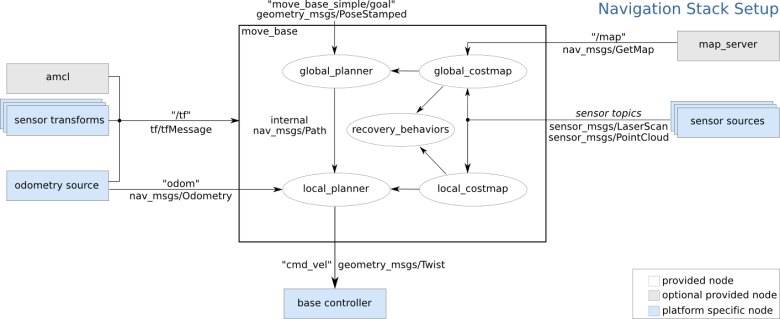
\includegraphics[width=\linewidth]{misc/overview_tf_small.png}
      \caption{amcl and navigation stack setup.}
      \label{fig:nav_stack}
\end{figure}

amcl\footnote{\url{http://wiki.ros.org/amcl}} package and navigation stack \footnote{\url{http://wiki.ros.org/navigation/Tutorials/RobotSetup}} have been installed in a catkin workspace and setup according to Fig. \ref{fig:nav_stack}. The simulation and parameter tuning were conducted on a Udacity virtual machine.

\subsection{Udacity Bot}
\label{subsec:udacity_bot}

The baseline mobile robot, Udacity Bot (UB), is developed using Xacro\footnote{\url{http://wiki.ros.org/xacro}} and Gazebo\footnote{\url{http://gazebosim.org/tutorials/?tut=ros_urdf}} definitions. The robot is constructed  with two-wheels, a Hokuyo laser scanner\footnote{\url{http://gazebosim.org/tutorials?tut=ros_gzplugins}}, and a camera attached a chassis. The structure of the robot is show in Fig. \ref{fig:udacity_bot}, and it visual appearance is given in Fig. \ref{fig:ub}  . The chassis is a 0.4, 0.2, 0.1 box, while the wheels are cylinders with radius 0.1 and length 0.05.  A differential drive has been attached to the left and right wheels, and configured via a Gazebo plugin. 

\begin{figure}[thpb]
      \centering
      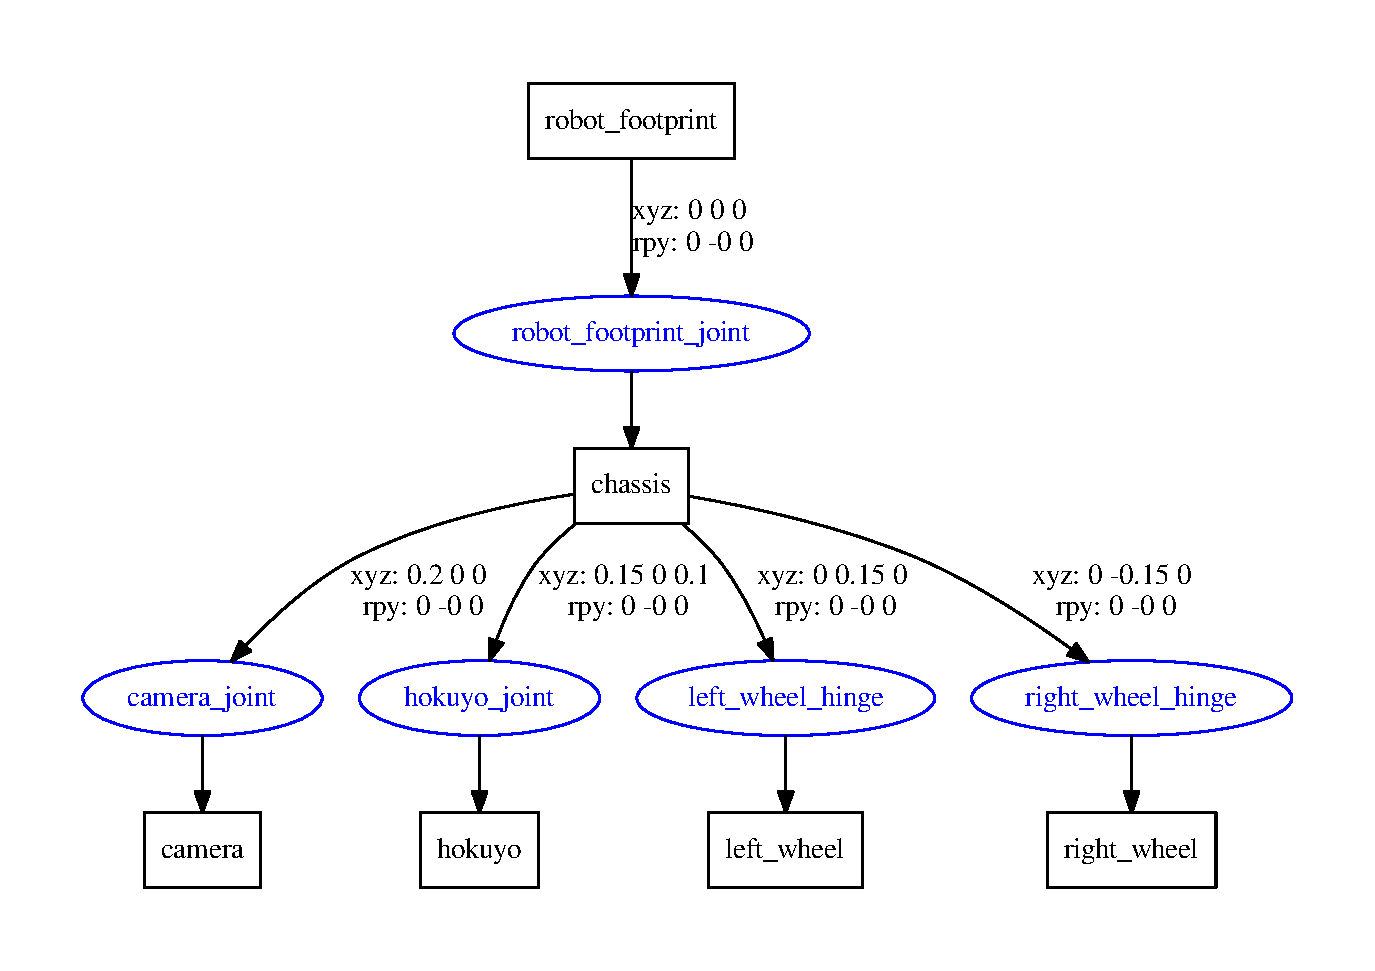
\includegraphics[width=\linewidth]{misc/udacity_bot.pdf}
      \caption{Structure of Udacity Bot.}
      \label{fig:udacity_bot}
\end{figure}

\begin{figure}[thpb]
      \centering
      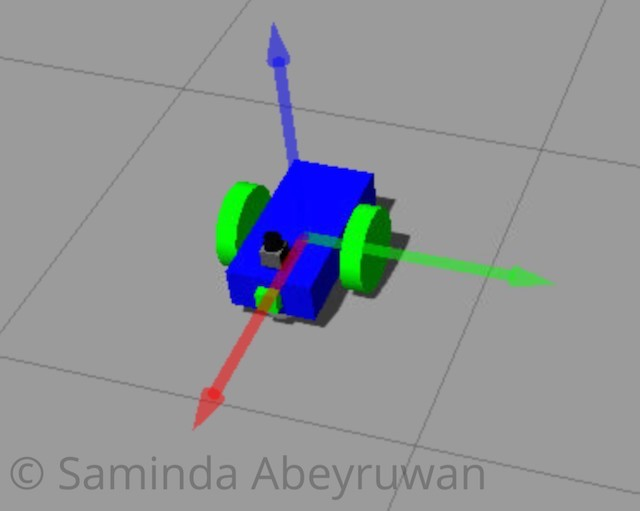
\includegraphics[width=\linewidth]{misc/ub_w.jpeg}
      \caption{Visual appearance of Udacity Bot.}
      \label{fig:ub}
\end{figure}

\subsection{Custom Robot Model}

The custom mobile robot, named Saminda Bot (SB), is a four-wheeled robot. The chassis is a box 0.2, 0.3, 0.1, while the wheels are cylinders with radius 0.05 and length 0.05. Similar to Sec. \ref{subsec:udacity_bot}, the robot is equipped with a Hokuyo laser scanner and a camera. The moment of inertia for each object shape has been calculated explicitly. A Skid Steering Drive has been attached to front/back left/right wheels and configured via Gazebo. Fig. \ref{fig:saminda_bot} shows the structure of Saminda Bot, and the visual appearance is given in Fig.  \ref{fig:sb}.

\begin{figure}[thpb]
      \centering
      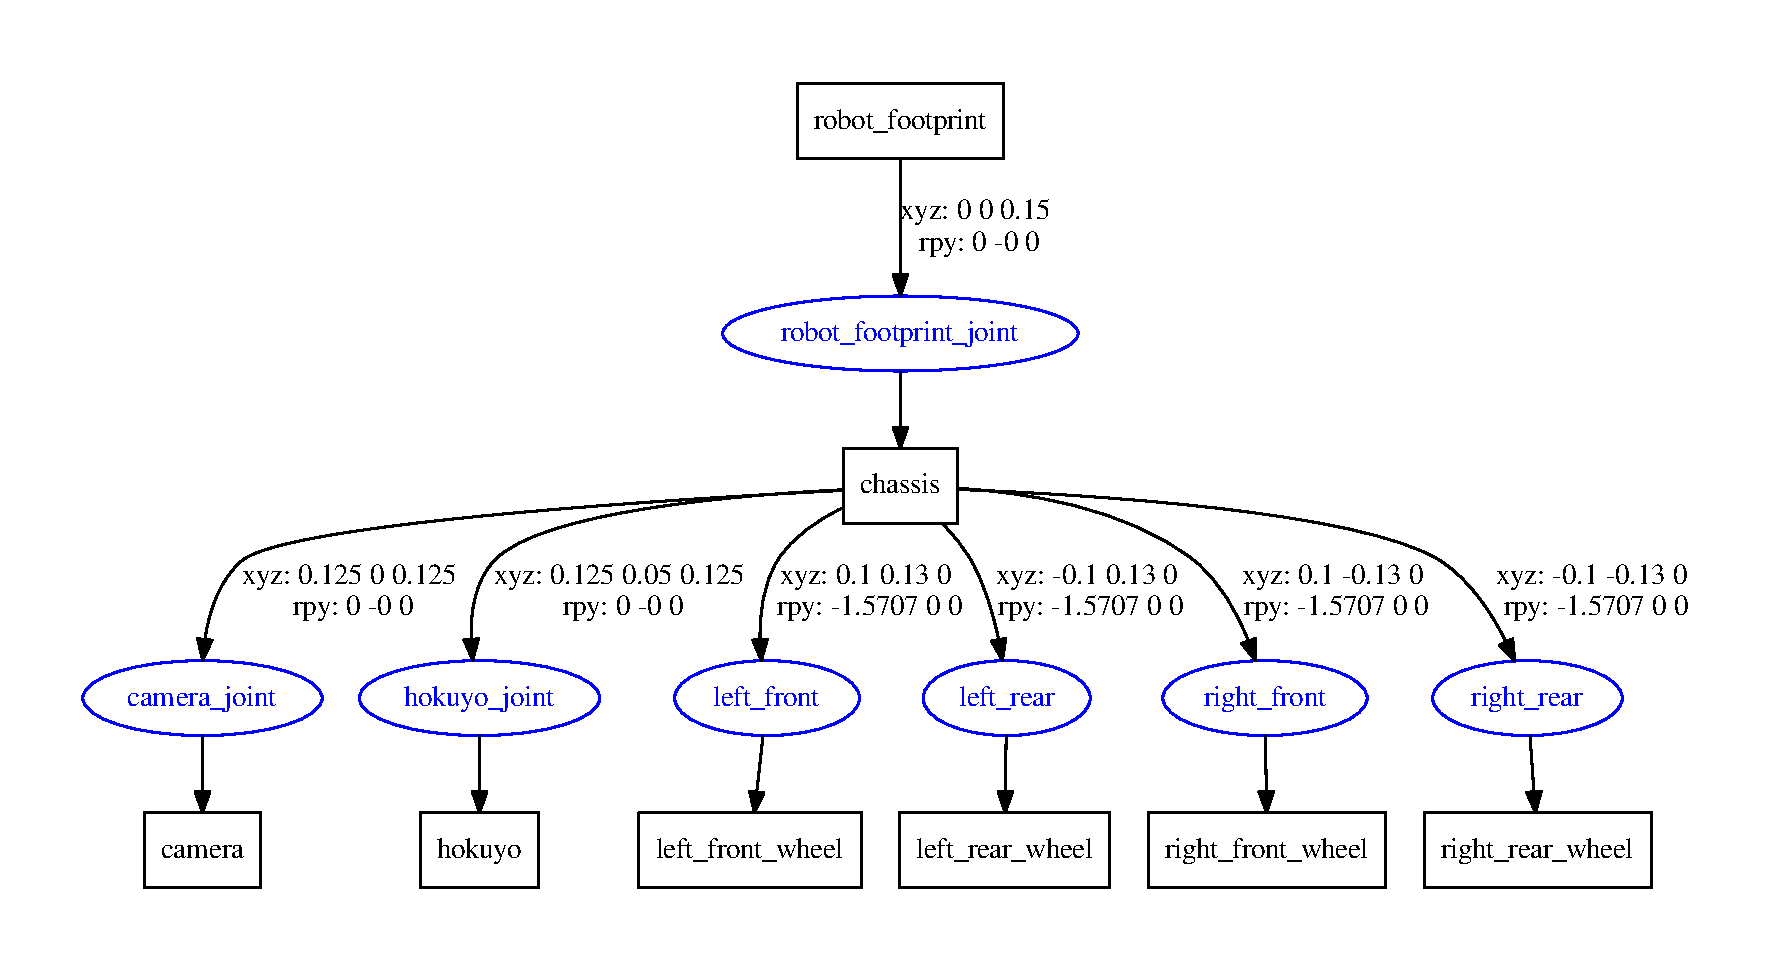
\includegraphics[width=\linewidth]{misc/saminda_bot.pdf}
      \caption{Structure of Saminda Bot.}
      \label{fig:saminda_bot}
\end{figure}

\begin{figure}[thpb]
      \centering
      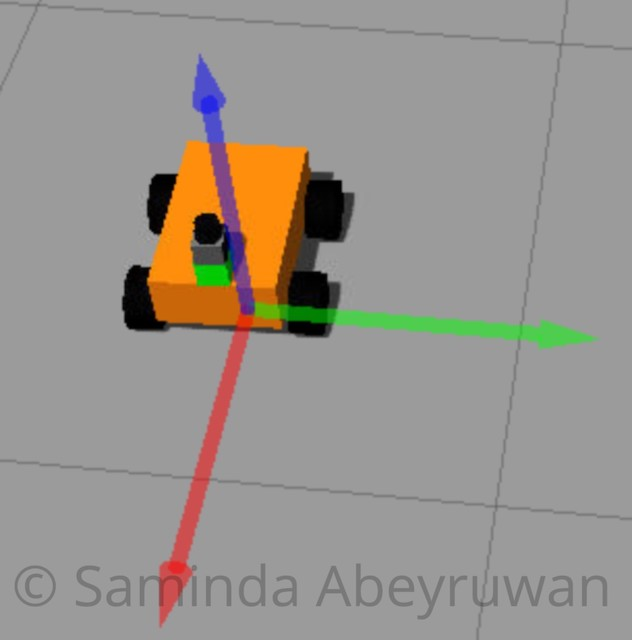
\includegraphics[width=\linewidth]{misc/sb_w.jpeg}
      \caption{Visual appearance of Saminda Bot.}
      \label{fig:sb}
\end{figure}

\subsection{ROS Packages}

The robots uses amcl package and ROS navigation stack to localize, plan a path, and move to the target pose.  In order to obtain successful robot behaviors, the parameters for the amcl, global planner, local planner, global costmap, and local costmap have been changed (Fig. \ref{fig:nav_stack}).   Both robots have used the same set of parameters to configure amcl (Table. \ref{tab:amcl_loc}).  The navigation stack parameters have been configured to match the characteristics of each robot. This has been the most time consuming part of the project, and the ROS tool \textit{rqt\_reconfigure} has been used extensively to view all parameters and configure them in real-time without restarting the simulation. The parameters for local planner and costmap common is given in Table \ref{tab:planner}. The global and local costmap parameters have not been changed.

\begin{table}[h]
\caption{AMCL parameters for both the UB and SB robots.}
\label{tab:amcl_loc}
\begin{center}
\begin{tabular}{|l|l|}
\hline
kld\_err & 0.05\\
kld\_z & 0.99\\
laser\_lambda\_short & 0.1 \\
laser\_likelihood\_max\_dist & 2.0\\
laser\_max\_beams & 60 \\
laser\_model\_type &  likelihood\_field\\
laser\_sigma\_hit & 0.2\\
laser\_z\_hit & 0.95\\
laser\_z\_short & 0.1 \\
laser\_z\_max & 0.05 \\
laser\_z\_rand & 0.5\\
max\_particles & 200\\
min\_particles & 20\\
odom\_alpha1 & 0.05\\
odom\_alpha2& 0.05\\
odom\_alpha3& 0.05\\
odom\_alpha4& 0.05\\
odom\_alpha5& 0.1\\
update\_min\_a & 0.1\\
update\_min\_d & 0.1 \\
initial\_pose\_x & 0\\
initial\_pose\_y & 0\\
initial\_pose\_a & 0\\
\hline
\end{tabular}
\end{center}
\end{table}

\begin{table}[h]
\caption{Navigation stack parameters for the UB and SB robots.}
\label{tab:planner}
\begin{center}
\begin{tabular}{|l||l|l|}
\hline
Local Planner Parameters & UB & SB\\
\hline
yaw\_goal\_tolerance &  0.05& 0.05\\
xy\_goal\_tolerance &  0.1& 0.1\\
pdist\_scale &  0.5& 0.5\\
gdist\_scale &  1.0& 1.0\\
max\_vel\_x &  0.5& 0.5\\
min\_vel\_x &  0.1& 0.1\\
max\_vel\_theta & 2.0 & 0.45\\
min\_vel\_theta &  -2.0& -0.45\\
acc\_lim\_theta &  5.0& 0.45\\
acc\_lim\_x & 2.0 & 0.25\\
acc\_lim\_y &  2.0& 0.25\\
min\_in\_place\_vel\_theta & 0.4 & 0.45\\
controller\_frequency &  10& 10\\
\hline
Costmap Common Parameters && \\
\hline
obstacle\_range  & 5.0 & 4.0 \\
raytrace\_range & 8.0 & 6.0\\
transform\_tolerance & 0.2 & 0.2\\
robot\_radius &  0.25& -\\
footprint &  - & [-0.2,-0.2],[-0.2,0.2],\\  
 &  &  [0.2, 0.2], [0.2,-0.2]\\
inflation\_radius & 0.3 & 0.2\\  
  &  & \\              
\hline
\end{tabular}
\end{center}
\end{table}



\section{Results}

Both the UB and SB robots have been localized and reach the benchmark target location. The two robots have different  physical characteristics, and the navigation stack has been configured such that both robots complete the navigation tasks. The UB robot is more responsive and reach the target pose within an average of 75 seconds, while the SB robots has taken on average 158 seconds. Figure \ref{fig:time_nav} shows sample traces of the completion of the navigation tasks. The SB robot has been configured to move conservatively than UB robot (Table \ref{tab:planner}). It has been observed that with the skid drive, if the robot turns faster, the amcl  injects particles into free space, and it has been controlled with slower motion. Figures \ref{fig:ub_motion} and \ref{fig:sb_motion} show the initial pose, three intermediate poses, and the final pose for the UB  and SB mobile robots.    

\begin{figure}
\centering
    \subfigure[Initial pose]
    {
        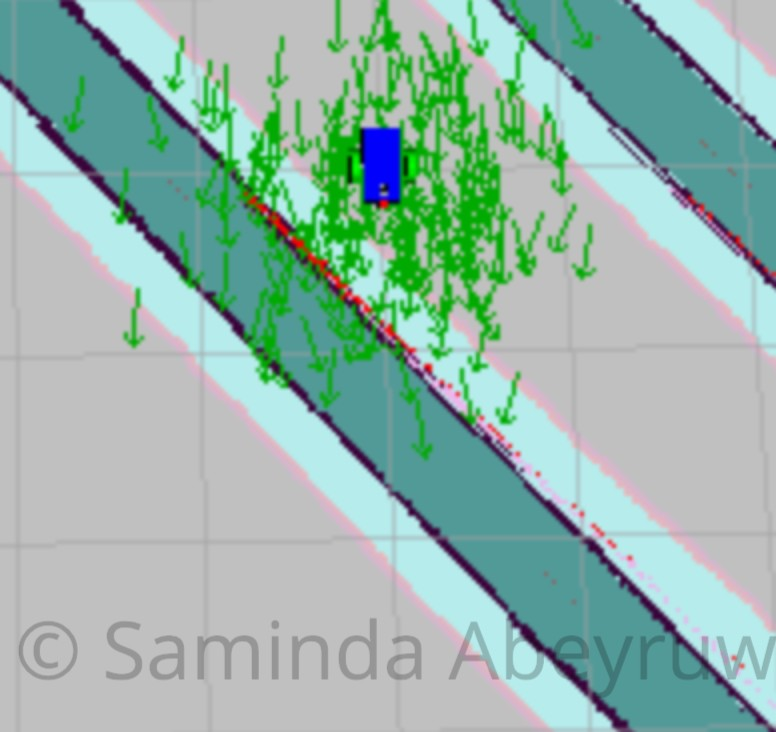
\includegraphics[width=0.6\linewidth]{misc/ub1}
        \label{fig:ub1}
    }
    \\
    \subfigure[Robot in motion (1)]
    {
        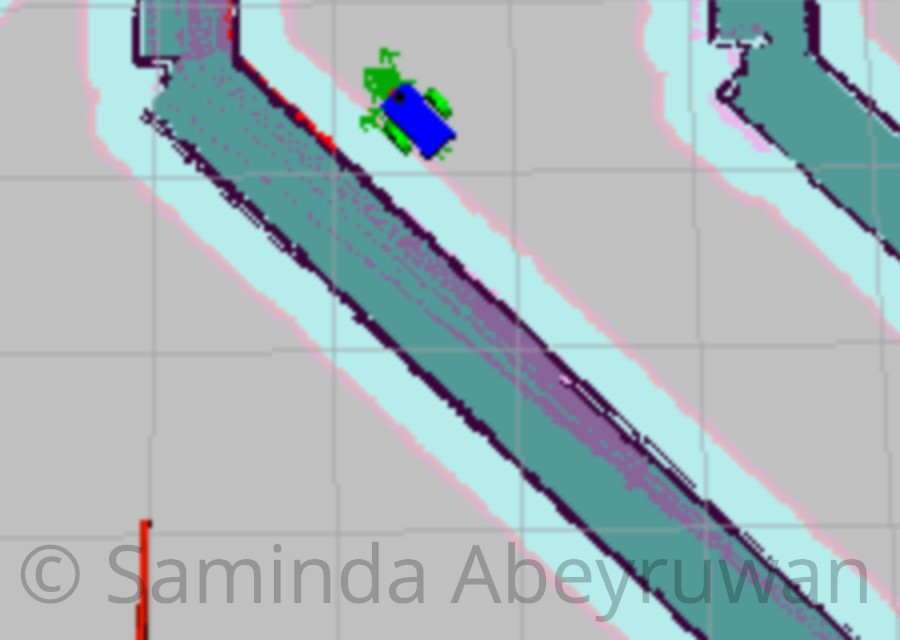
\includegraphics[width=0.6\linewidth]{misc/ub2}
        \label{fig:ub2}
    }
    \\
    \subfigure[Robot in motion (2)]
    {
        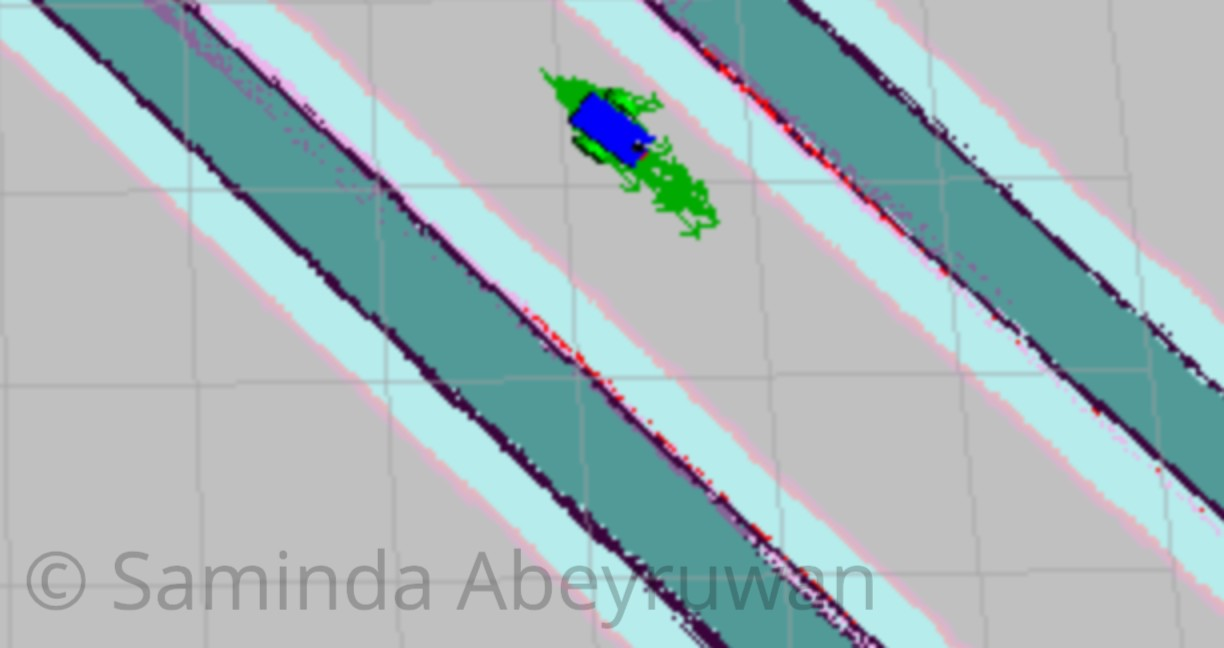
\includegraphics[width=0.6\linewidth]{misc/ub3}
        \label{fig:ub3}
    }
    \\
    \subfigure[Robot in motion (3)]
    {
        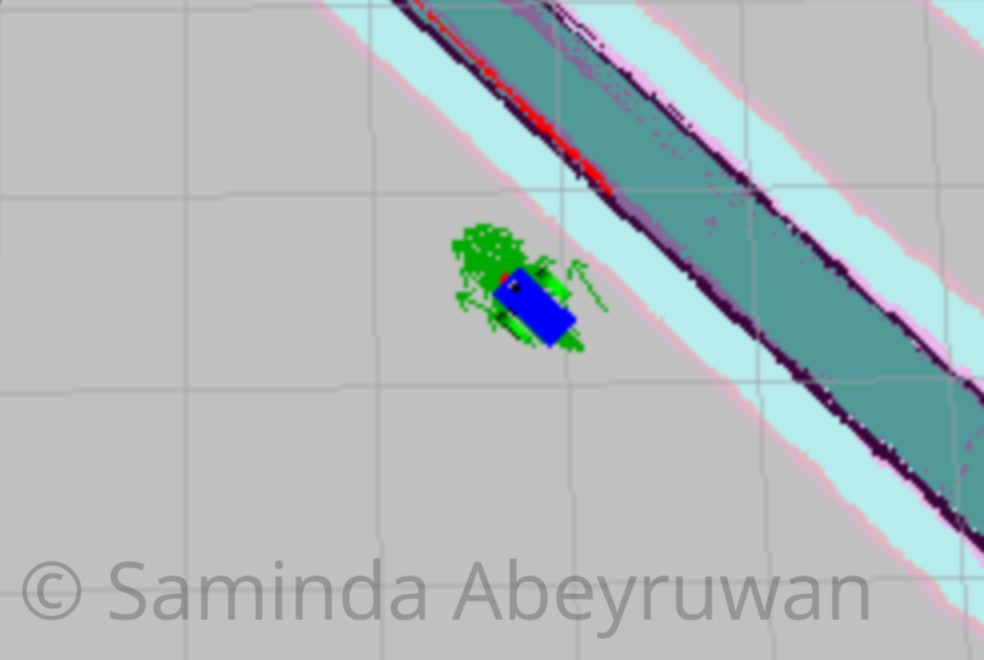
\includegraphics[width=0.6\linewidth]{misc/ub4}
        \label{fig:ub4}
    }
    \\
    \subfigure[Final pose]
    {
        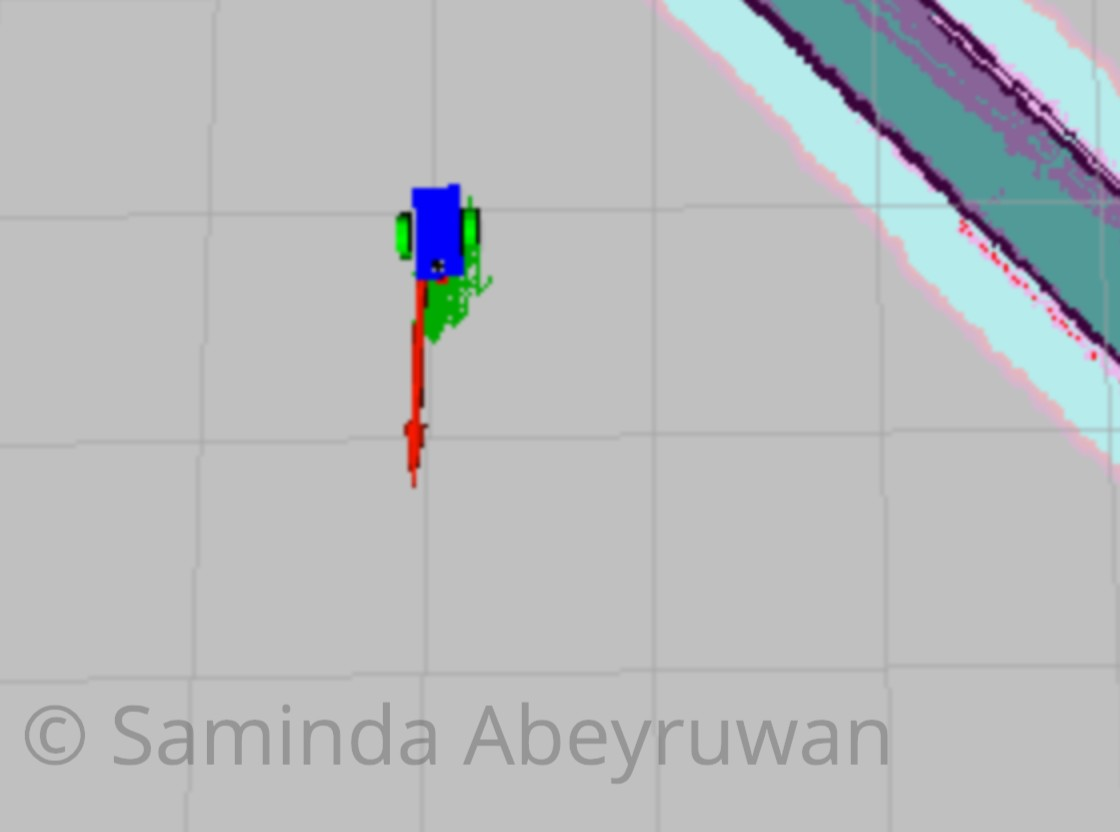
\includegraphics[width=0.6\linewidth]{misc/ub5}
        \label{fig:ub5}
    }
    \caption{Robot motion for the UB robot.}
    \label{fig:ub_motion}
\end{figure}


\begin{figure}
\centering
    \subfigure[Initial pose]
    {
        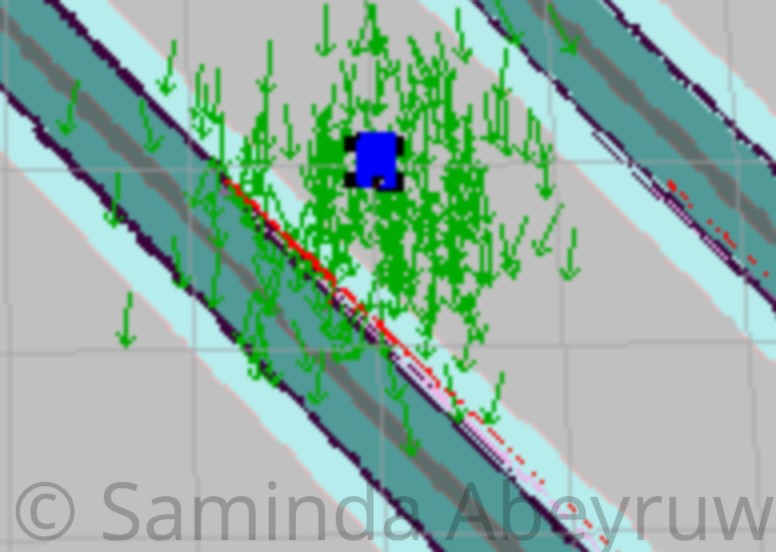
\includegraphics[width=0.6\linewidth]{misc/sb1}
        \label{fig:sb1}
    }
    \\
    \subfigure[Robot in motion (1)]
    {
        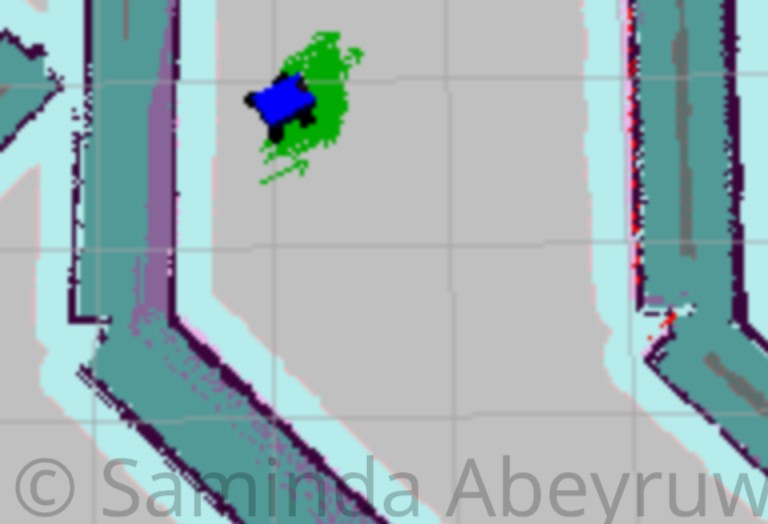
\includegraphics[width=0.6\linewidth]{misc/sb2}
        \label{fig:sb2}
    }
    \\
    \subfigure[Robot in motion (2)]
    {
        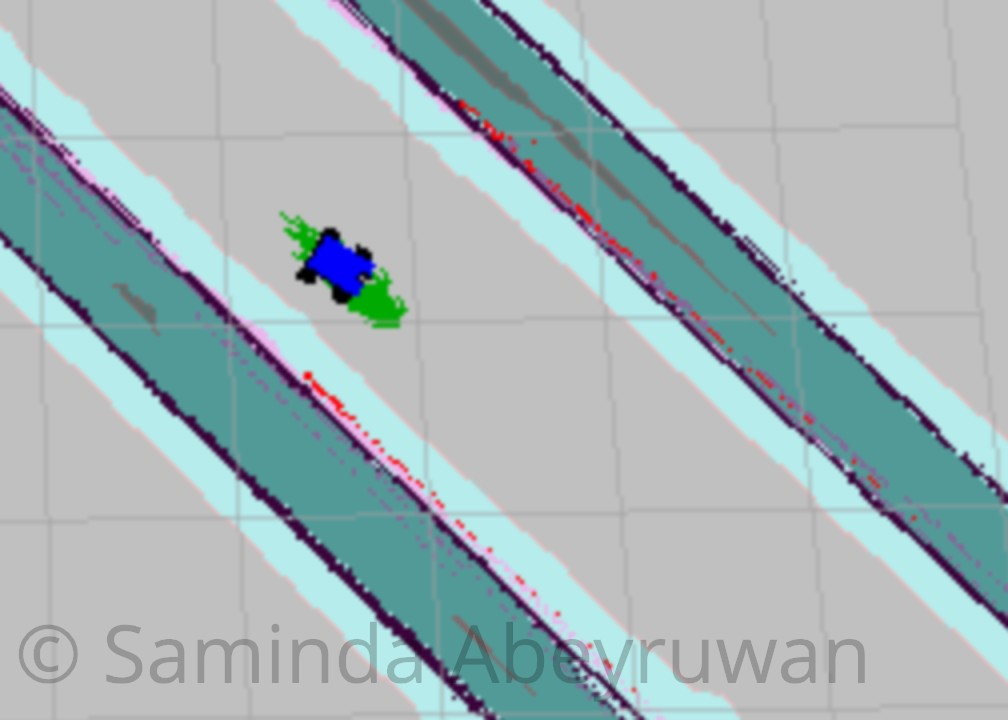
\includegraphics[width=0.6\linewidth]{misc/sb3}
        \label{fig:sb3}
    }
    \\
    \subfigure[Robot in motion (3)]
    {
        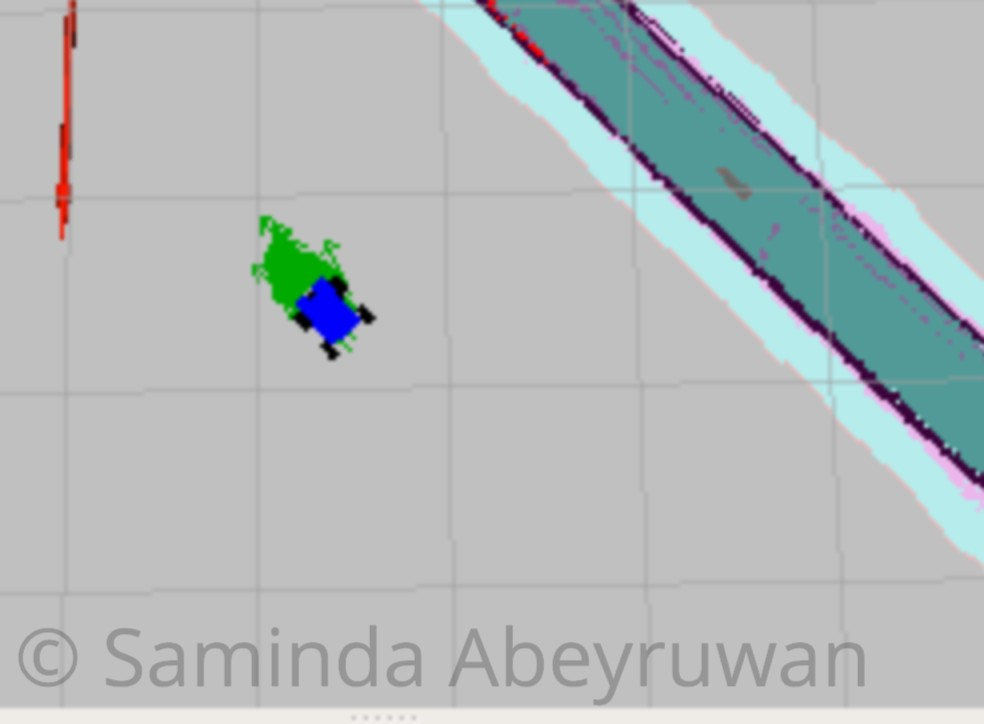
\includegraphics[width=0.6\linewidth]{misc/sb4}
        \label{fig:sb4}
    }
    \\
    \subfigure[Final pose]
    {
        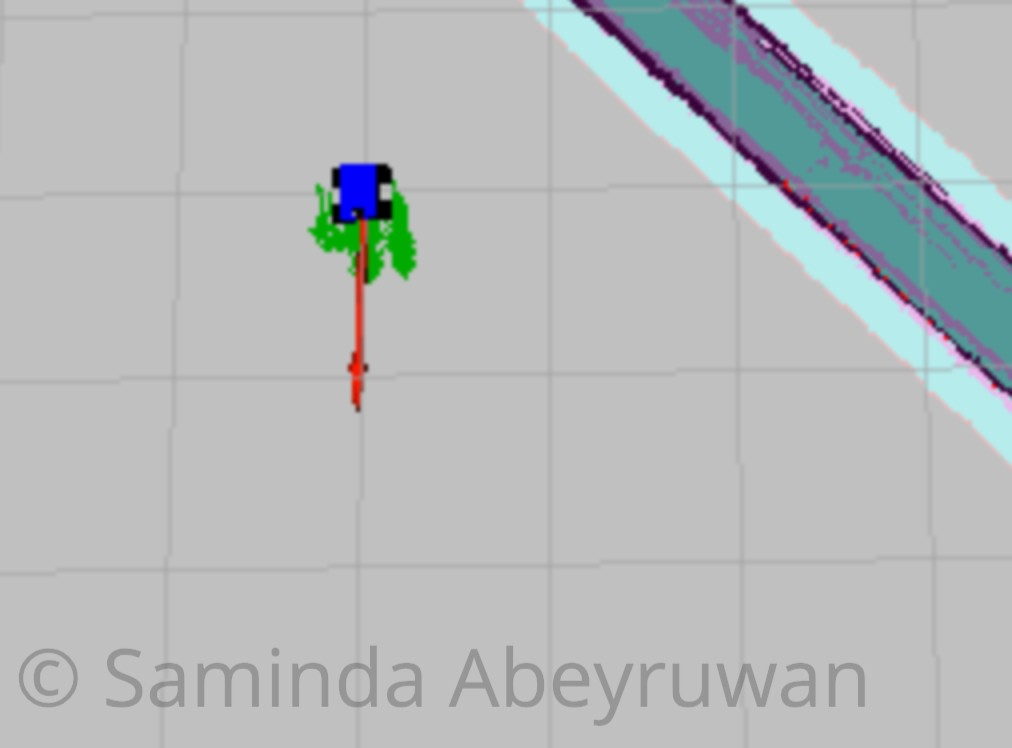
\includegraphics[width=0.6\linewidth]{misc/sb5}
        \label{fig:sb5}
    }
    \caption{Robot motion for the SB robot.}
    \label{fig:sb_motion}
\end{figure}

\begin{figure}
\centering
    \subfigure[A time trace for the UB navigation task]
    {
        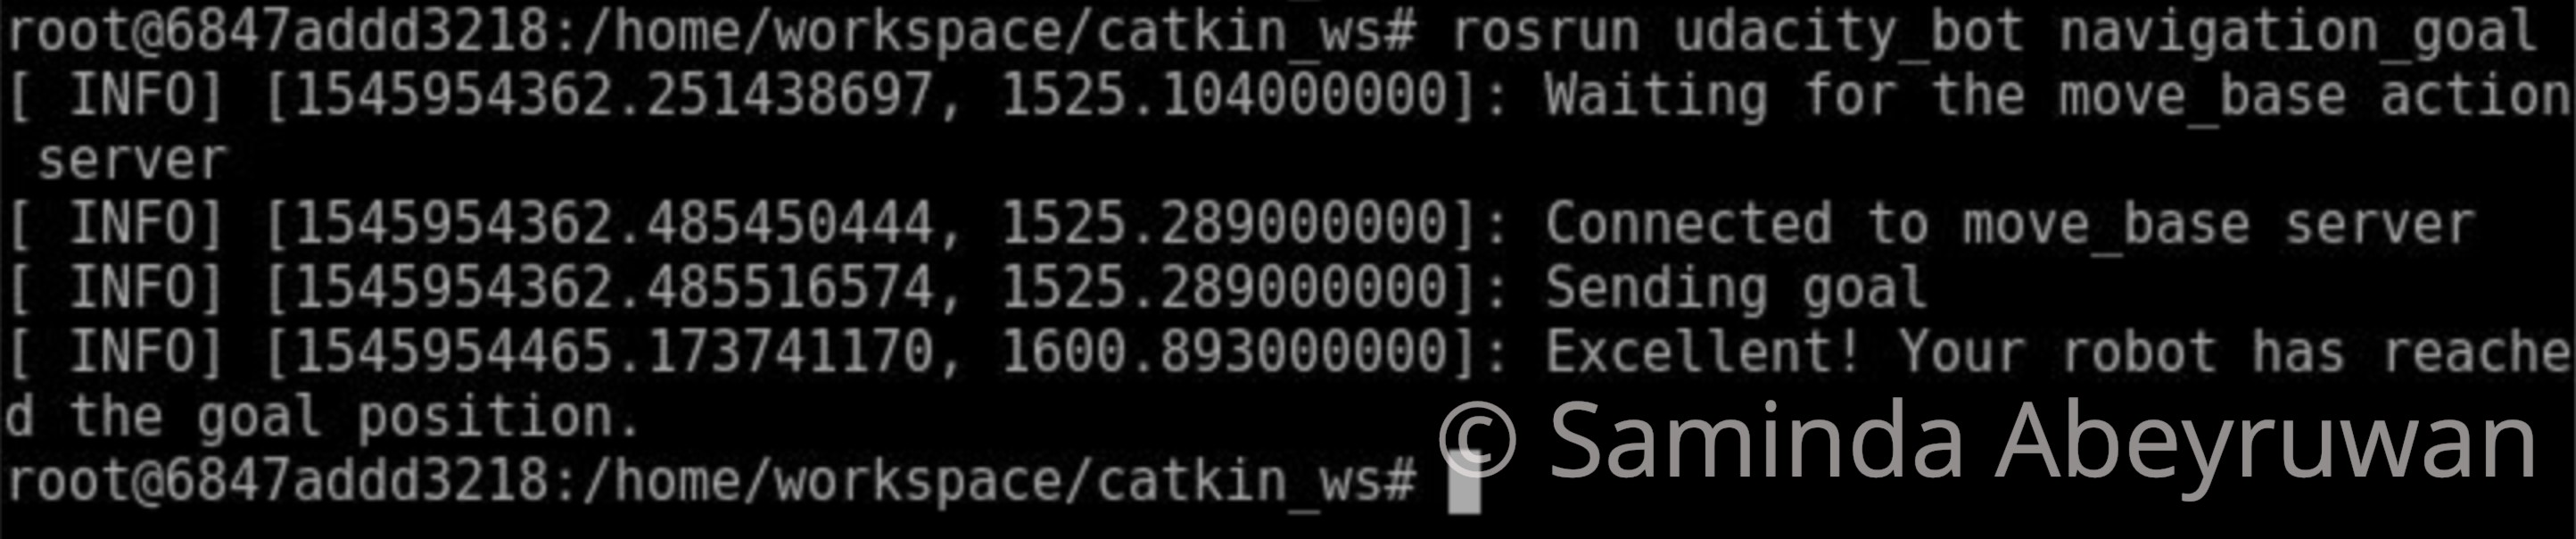
\includegraphics[width=\linewidth]{misc/ub_t1}
        \label{fig:ub1}
    }
    \\
    \subfigure[A time trace for the SB navigation task]
    {
        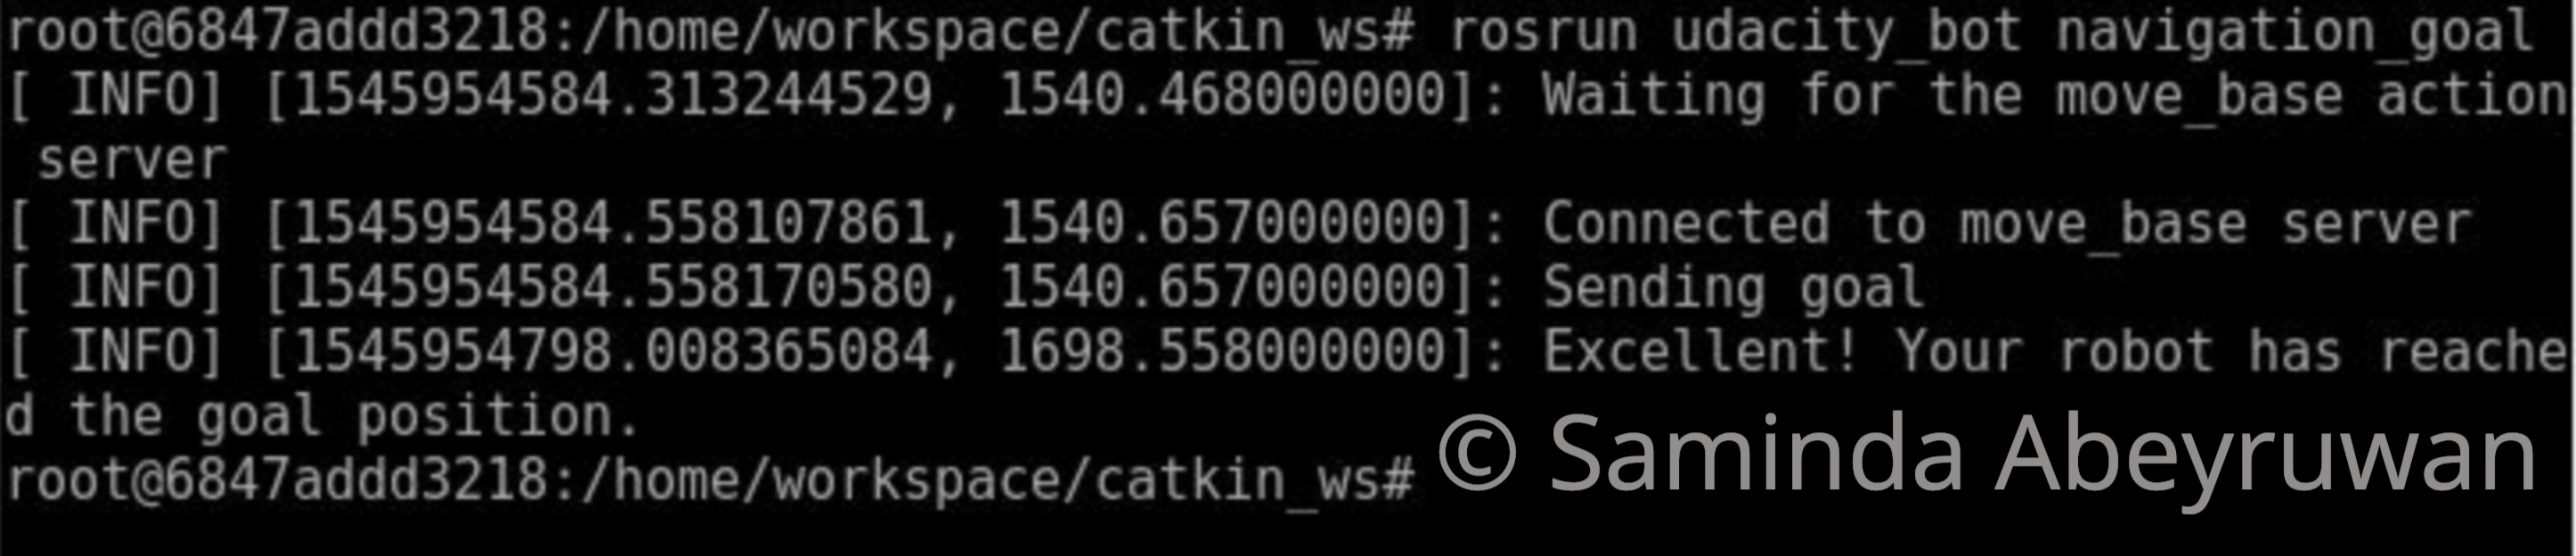
\includegraphics[width=\linewidth]{misc/sb_t1}
        \label{fig:ub2}
    }   
    \caption{Time traces of navigation task.}
    \label{fig:time_nav}
\end{figure}



\section{Discussion}

Both robots have successfully localized and completed the navigation tasks. Due to the robots physical characteristics and different drives, the steering performance have empirically shown to be significantly different.  Due to some noise of the simulation, the robots have not taken the same path to the goal, and some paths were suboptimal and have taken more time to reach the target pose. amcl has the capability to solve the kidnapped robot problem; it has been observed that the robots were able to localize and move to the target pose.   


\section{Conclusion / Future work}

The project evaluates the functions of the ROS navigation stack and amcl packages on two simulated mobile robots. It has been shown that the robots were successfully localized and completed the navigation tasks. All tasks have been experimented in simulation. amcl package and the navigation stack provide plethora of parameters that can be used to tune for the different robot platforms. It is also interesting  to integrate the packages on real hardware and tune for the real world constrains. This project evaluated only one scenarios introduced in Sec. \ref{sec:introduction}. It is advantageous to simulate other scenarios and use in real world robotic problems. 

%This section is intended to summarize your report. Your summary should include a recap of the results, did this project achieve what you attempted, and is this a commercially viable product? 
%For Future work,address areas of work that you may not have addressed in your report as possible next steps. For future work, this could be due to time constraints, lack of currently developed methods / technology, and areas of application outside of your current implementation. Again, avoid the use of the first-person.

\bibliography{bib}
\bibliographystyle{ieeetr}

\end{document}